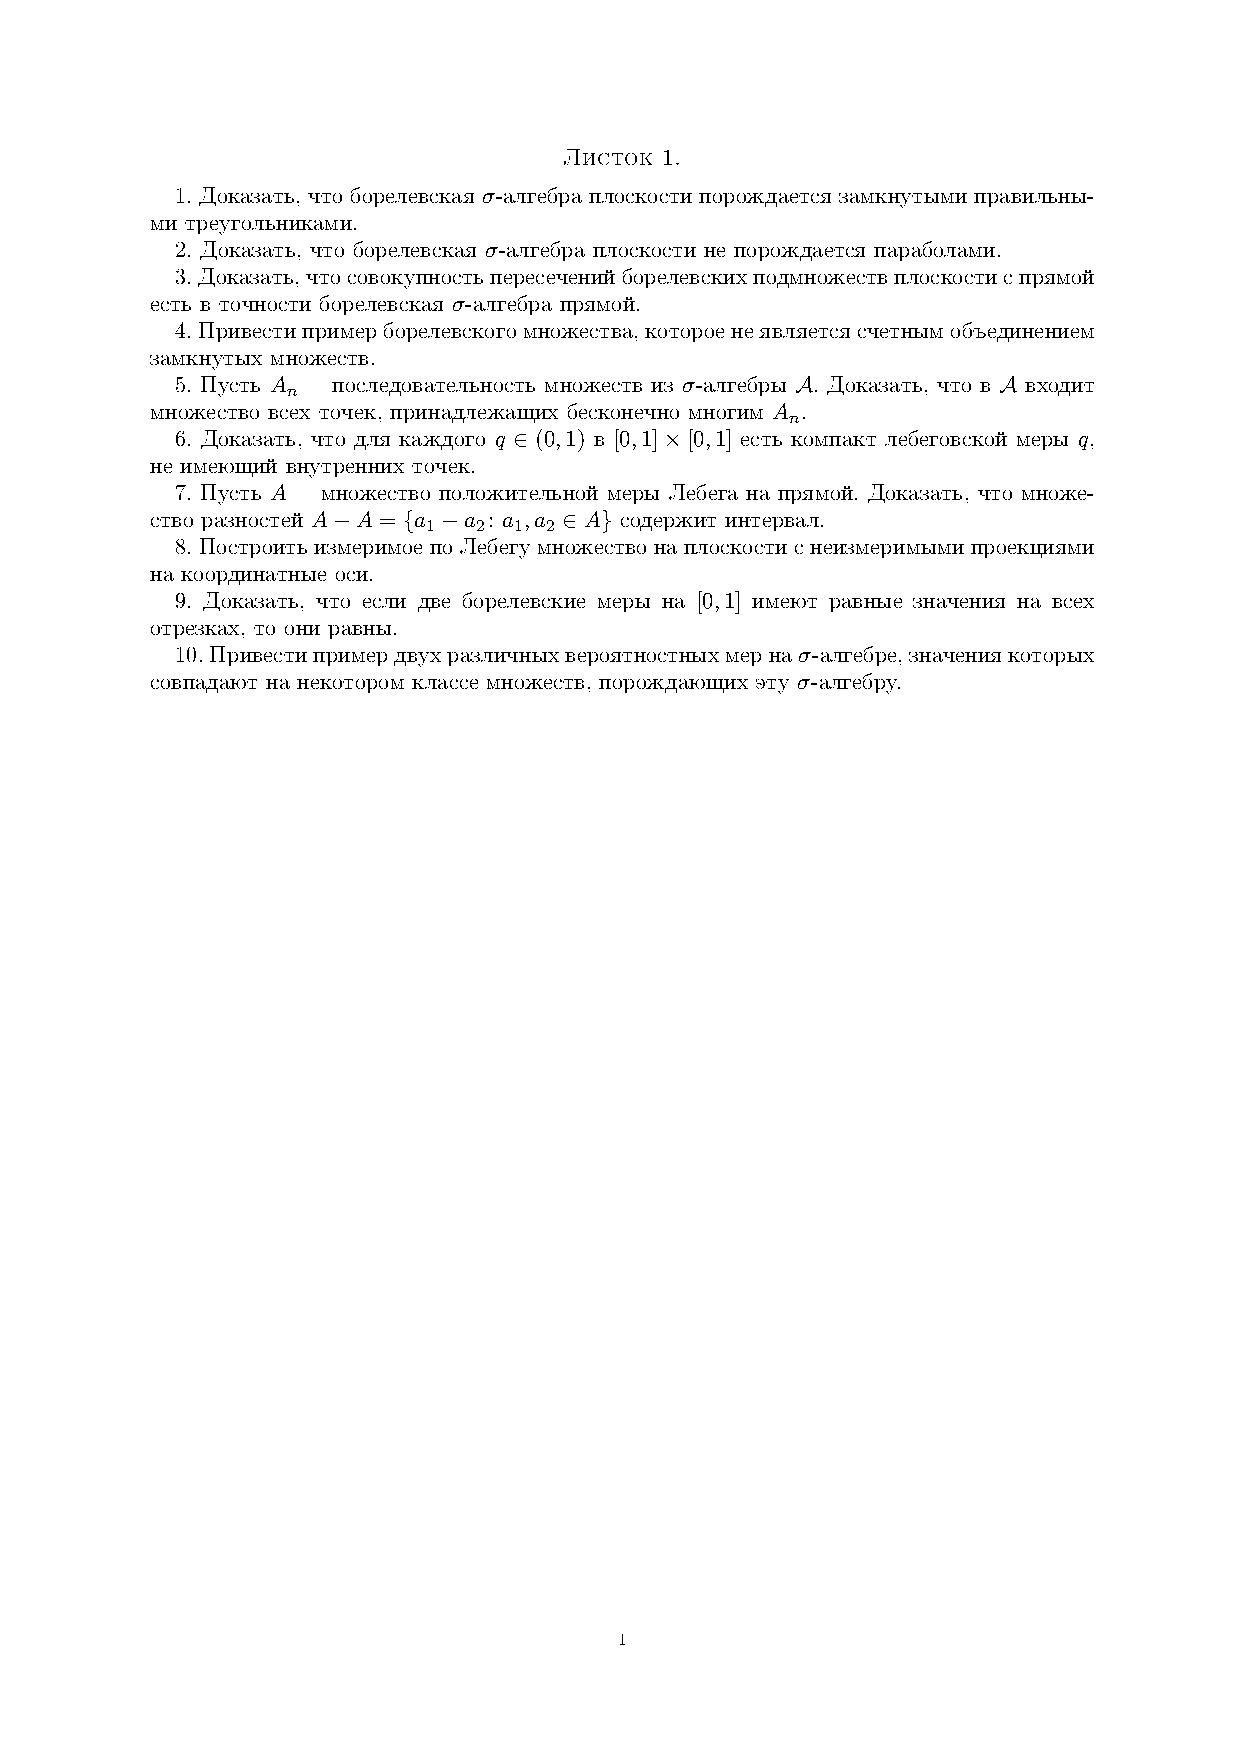
\includepdf{Tasks/listok-matan1}
\newpage
\section*{Решения}
\subsection*{Задача 1}
	Заметим что борелевская $\sigma$-алгебра, тогда мы докажем что квадрат можно замостить правильными треугольниками. Рассмотрим треугольную сетку на плоскости из треугольников со стороной 1 и квадрат нарисованный поверх нее. Выберем в множество $A_1$ треугольники которые целиком лежат в квадрате, далее рассмотрим сетку в 2 раза меньшую и выберем в множество $A_2$ треугольники с вдвое меньшей стороной, лежащие внутри квадрата и не пересекающиеся с $A_1$ и так далее. Таким образом каждая точка войдет в какой-то треугольник и $[0,1]^2 = \bigcup\limits_{i=1} A_i$. Таким образом мы доказали, что борелевскую $\sigma$-алгебру плоскости можно породить треугольниками.


\subsection*{Задача 2}
	Заметим, что парабола пересекается с прямой не более чем в двух точках, тогда если рассмотреть любе счетное число парабол, то они пересекаются с прямой не более чем в счетном числе точек, а следовательно мы не можем представить интервал в виде объединения парабол, а следовательно не все множества на $\mathbb{R}$ могут быть представлены через параболы.


\subsection*{Задача 3}
	$A = \{V_1 \cap \mathbb{R}\ |\ V_1 \subset B(\mathbb{R}^2)\}$ -- $\sigma$-алгебра на $\mathbb{R}$
	\begin{gather*}
	\mathbb{R} \in A\quad (\mathbb{R}^2 \cap \mathbb{R} = \mathbb{R})\\
	U_1 \in A\ \Rightarrow\ U_1 \backslash \mathbb{R} = V_1 \cap \mathbb{R} \backslash \mathbb{R} = (\mathbb{R}^2 \backslash V_1) \cap \mathbb{R}\quad \mathbb{R}^2 \backslash V_1 \text{ -- борелевское, а следовательно } U_1 \backslash \mathbb{R} \in A\\
	U_1, U_2, \ldots \in A\qquad U_i = V_i \cap \mathbb{R}\\
	\bigcup\limits_{i=0}^{\infty} (U_i) = \bigcup\limits_{i = 0}^{\infty} (V_i \cap \mathbb{R}) = \left(\bigcup\limits_{i = 0}^{\infty} V_i\right) \cap \mathbb{R} \subset \text{борелевского}
	\end{gather*}
	Тогда $\mathcal{A} \subset A$, где $\mathcal{A}$ -- борелевская $\sigma$-алгебра прямой (так как она является наименьшей $\sigma$-алгеброй), содержащей все открытые множества в $\mathbb{R}$\\
	$A' = \{ W_1 \subset \mathbb{R}^2\ |\ W_1 \cap \mathbb{R} \text{ -- борелевское множество в } \mathbb{R}\}$\\
	$A'$ -- $\sigma$-алгебра на $\mathbb{R}^2$
	\begin{gather*}
	\mathbb{R}^2 \subset A'\quad \mathbb{R}^2 \cap \mathbb{R} = \mathbb{R} \subset B(\mathbb{R})\\
	W_1 \subset A'\ \Rightarrow\ W_1 \cap \mathbb{R} \subset \mathcal{A}\\
	\vdots
	\end{gather*}
	Все открытые множества в $\mathbb{R}^2 \subset A'$, так как $W_1 \cap \mathbb{R} = U_1 \in \mathcal{A}$ (где $W_1, U_1$ -- открыты)\\
	$A'$ -- $\sigma$-алгебра, следовательно $B(\mathbb{R}) \subset A'$, откуда $A' \cap \mathbb{R} \supset A$, $A \subset A' \cap \mathbb{R} \subset \mathcal{A}$, а следовательно $A = \mathcal{A}$

\begin{comment}
	Докажем что совокупность пересечений борелевских подмножеств плоскости с прямой есть в точности борелевская $\sigma$-алгебра прямой\\
	\begin{gather*}
	A = \{B_2 \cap \mathbb{R}\ |\ B_2 \text{-- борелевское подмножество } \mathbb{R}^2\}\quad A -- \sigma\text{-алгебра}\\
	\mathbb{R}^2 \cap \mathbb{R} = \mathbb{R} \in A\\
	A_1 \in A\ \Leftrightarrow\ A_1 = B_2 \cap \mathbb{R}\ \Rightarrow
	\end{gather*}
\end{comment}


\subsection*{Задача 4}
	Борелевское множество не является счетным объединением замкнутых множеств.\\
	$\mathbb{R} \backslash \mathbb{Q}$ -- борелевское множество
	\begin{gather*}
	\mathbb{R} \backslash q = (-\infty, q) \cup (q,+\infty)\quad q \in \mathbb{Q}\\
	\bigcap\limits_{i=1}^{\infty} \mathbb{R} \backslash q = \mathbb{R} \backslash \mathbb{Q}
	\end{gather*}
	$\mathbb{Q}$ (это счетное объединение замкнутых множеств) так как точка $q = \mathbb{R} \backslash (-\infty, q) \cup (q, +\infty)$ замкнута\\
	Пусть $\mathbb{R} \backslash \mathbb{Q} = \bigcup\limits_{i=1}^{\infty} z_i$ ($z_i$ -- замкнутое множество)\\
	Тогда $\mathbb{Q} = \bigcap\limits_{i=1}^{\infty} (\mathbb{R} \backslash z_i)$ ($\mathbb{R} \backslash z_i$ -- открытое множество)
	\vskip 0.1in
	\myuline{Теорема Бэра} Семейство $A_n$ --всюду плотные открытые множества, тогда $\bigcap A_n$ -- всюду плотно
	\vskip 0.1in
	Если $\mathbb{Q}$ -- пересечение открытых, то они содержат рациональные точки, а следовательно эти множества всюду плотные
	\begin{gather*}
	\mathbb{Q} \cap (\mathbb{R} \backslash \mathbb{Q}) = \left(\bigcap\limits_{i=1}^{\infty} \mathbb{R} \backslash z_i \right) \cap \left(\bigcap\limits_{j=1}^{\infty} \mathbb{R} \backslash q_j\right) = \varnothing
	\end{gather*}
	Противоречие, следовательно $\bigcap\limits_{i=1}^{\infty} (\mathbb{R} \backslash z_i)$ не всюду плотно, следовательно $\ne \mathbb{Q}$


\subsection*{Задача 5}
	$X = \bigcap\limits_{n=1}^{\infty} \bigcup\limits_{k=n}^{\infty} A_k$\\
	Докажем, что все элементы $X$ удовлетворяют условию
	\begin{enumerate}
	\item \begin{gather*}
		x \in X\ \Rightarrow\ \forall N\ \exists n > N:\ x \in A_n\\
		\forall N:\ x \in \bigcup\limits_{k=n}^{\infty} A_n\ \Rightarrow\ x \in \bigcap\limits_{n=1}^{\infty} \bigcup\limits_{k=n}^{\infty} A_k
	\end{gather*}
	\item
		$x \in X$, но при этом $x$ принадлежит конечному числу множеств, а следовательно $\exists N\ \forall n > N: x \notin A_n\ \Rightarrow\ x \notin \bigcup\limits_{k=n}^{\infty} A_k$, следовательно $x \notin \bigcap\limits_{n=1}^{\infty} \bigcup\limits_{k=n}^{\infty} A_k$, но это равносильно тому, что $x \in X$
	\end{enumerate}


\subsection*{Задача 6}
	$K = ([0,1] \backslash \bigcup\limits_{n=1}^{\infty} I_n) \times ([0,1] \backslash \bigcup\limits_{n=1}^{\infty} I_n)$.\\
	Зафиксируем $\varepsilon = \sqrt{q} + 1$, построим множество лебеговской меры $1 - \varepsilon$, пусть есть последовательность $\{a_n\}:\ a_0 = 1,\ a_0 > a_1 > \ldots$ и $\lim\lim\limits_{n \to \infty} a_n = 1 - \varepsilon$. Рассмотрим отрезок и будем из него выреать участки длины $\frac{a_{n-1} - a_{n}}{2^{n-1}}$ (на $n$ шаге), тогда
	\begin{gather*}
		\lambda(K) = \inf(\sum\limits_{i=1}^{\infty} \lambda(u_i),\ K \subset \bigcup\limits_{i=1}^{\infty} u_i) = 1 - \lambda([0,1]\backslash K) = \varepsilon
	\end{gather*}
	$\lambda([0,1] \backslash K) = 1 - \varepsilon$, так как частичные суммы равны равны $l_0-l_1, l_0-l_2, \ldots, l_0-l_n$ $1-(1-\varepsilon) = \varepsilon$\\
	Множество $K$ замкнуто ($[0,1]\backslash K$ открыто как счетное объединение открытых) и ограничено, а следовательно не имеет внутренних точек, так как мы выкинули всюду плотное множество.\\
	Рассмотрим $K \times K \subset [0,1] \times [0,1]$\\
	$\lambda(K \times K) = |x| - 2 \varepsilon + \varepsilon^2 = (\varepsilon - 1)^2$\\
	$-2\varepsilon$ так как мы выкинули $S$ всех "полосок" по горизонтали и вертикали $(a_0 - a_1 + 2 \frac{a_1 - a_2}{2} + 2 \cdot \ldots) = \varepsilon$\\
	$+\varepsilon^2$ так как мы добавляем $S$ пересечения этих полосок $(a_0 - a_1)(a_0 - a_1 + 2 \frac{a_1 - a_2}{2} + 2 \cdot \ldots) + \frac{a_1-a_2}{2}(a_0 - a_1 + 2 \frac{a_1 - a_2}{2} + 2 \cdot \ldots) + \ldots = (a_0 - a_1) \varepsilon + (\frac{a_0 - a_1}{2})\varepsilon + \ldots = \varepsilon^2$


\subsection*{Задача 7}
	Докажем что $\exists \varepsilon > 0: (-\epsilon, \epsilon) \subset A - A$\\
	Если $\mu(A) > 0$, то существуют компакты для которых выполнено что $U_2 \subset A \subset U_1$ и $\mu(U_1 \backslash U_2) < \frac{1}{3}\mu(A)$, тогда
	\begin{gather*}
		\mu(U_2) > \mu(A) - \mu(A \backslash U_2) \geqslant \mu(A) - \mu(U_1 \backslash U_2) > \frac{2}{3} \mu(A)\\
		\mu(U_1) \leqslant \mu(A) + \mu(U_1 \backslash A) \leqslant \mu(A) + \mu(U_1 \backslash U_2) < \frac{4}{3} \mu(A)\\
		2\mu(U_2) > \mu(U_1)
	\end{gather*}
	\vskip 0.2in
	Теперь рассмотрим $U_1, U_2$ и докажем, что $\exists \varepsilon > 0:\ \forall \delta \in (-\epsilon, \epsilon):\ (U_2 + \delta) \subset U_1$\\
	$U_1 = \bigsqcup\limits_{i=1} I_i$ -- дизъюнктное объединение интервалов $\{I_n\}$ -- открытое покрытие $U_2$, следовательно $\exists N:\ U'_1 = \bigsqcup\limits_{i=1}^{N} I_i\ U_2 \subset U'_1$\\
	Покажем, что $I_n \cap K$ -- компакт ($\forall n = 1,\ldots,N$)\\
	Пусть $I_n = [a_n, b_n]$ и $U_2 \cap I_n = u_n$, заметим что $a_n,b_n \notin U_2$, так как $a_n,b_n \notin U'_1$, откуда $u_n = U_2 \cap [a_n, b_n]$ -- ограниченное замкнутое подмножество прямой, а следовательно $u_n$ -- компакт и $\inf u_n, \sup u_n \in u_n$.\\
	Обозначим $\varepsilon_n^{1} = \inf u_n - a > 0$ и $\varepsilon_n^{2} = b - \sup u_n > 0$, $\varepsilon_n = \min (\varepsilon_n^{1}, \varepsilon_n^{2}) > 0$ и $\forall \delta \in (-\varepsilon_n, \varepsilon_n):\ u_n + \delta \subset I_n$, следовательно для $\varepsilon = \min \{\varepsilon_n\} > 0$ выполнено что $\forall \delta \in (-\varepsilon, \varepsilon):\ \forall n \in (1,\ldots,N):\ u_n + \delta \subset I_n$. Откуда следует что $U_2 + \delta \subset U'_1 \subset U_1$
	
	\begin{gather*}
		\mu(U_2 \cap U_2 + \delta) = \mu(U_2) + \mu(U_2 + \delta) - \mu(U_2 \cup (U_2 + \delta)) \geqslant 2\mu(U_2) - \mu(U_2) > 0
	\end{gather*}



\subsection*{Задача 8}
	Известно, что существует хотя бы одно неизмеримое множество на прямой (например множество Витали), обозначим такое множество как $A$. Построим тогда множества $B_1 = \{(x,y)\ |\ x \in A, y = 0\}$ и $B_2 = \{(x,y)\ |\ x = 0,\ y \in A \}$. Тогда множество $B = B_1 \cup B_2$ удовлетворяет условию, ведь $B$ измеримо, так как это объединение подмножеств двух прямых. Проекции же, имеющие вид $A \cup \{0\}$, являются неизмеримыми.


\subsection*{Задача 9}
	Назовем класс множеств, на которых две меры имеют равные значения -- $A$, заметим что если выбрать в $A$ сходящуюся последовательность отрезков $B_1, B_2, B_3, \ldots$, то $\lim\limits_{n \to \infty}(\mu_1(B_n)) = \lim\limits_{n \to \infty}(\mu_2(B_n))$, а следовательно $\lim\limits_{n \to \infty}(\mu_1(B_n)) = B \in A$. Тогда заметим, что $\forall \{B_n\} \in A,\ B_1 \subset B_2 \subset B_3 \subset \ldots:\ \bigcap\limits_{n=1}^{\infty} B_n \in A$, то есть это монотонный класс, а следовательно для него выполнена теорема о монотонном классе, то есть данные две меры порождают какую-то $\sigma$-алгебру с равными значениями, а следовательно можно выбрать в них минимальную $\sigma$-алгебру.


\subsection*{Задача 10}
	\begin{gather*}
		\mu_1(1) = \mu_1(3) = 0\quad \mu_1(2) = \mu_1(4) = \frac{1}{2}\\
		\mu_2(1) = \mu_2(2) = \mu_2(3) = \mu_2(4) = \frac{1}{4}\\
		\sum\limits_{k=1}^{4} \mu_1(k) = \sum\limits_{k=1}^{4} \mu_2(k) = 1
	\end{gather*}
	Пусть $A = \{1,2,3,4\}$. $\sigma$-алгебра -- множество всех подмножеств в $A$, она порождается $\{1,2\}$ и $\{2,3\}$
	\begin{gather*}
		\mu_1(\{1,2\}) = \frac{1}{2} = \mu_2(\{1,2\})\\
		\mu_1(\{2,3\}) = \frac{1}{2} = \mu_2(\{2,3\})\\
		\mu_1(1) \ne \mu_2(1) \text{ меры различны}
	\end{gather*}
	
